%%%%%%%%%%%%%%%%%%%%%%%%%%%%%%%%%%%%%%%%%%%%%%%%%%%%%%%%%%%%%%%%%%%%%%%%%%%%%%%%
%2345678901234567890123456789012345678901234567890123456789012345678901234567890
%        1         2         3         4         5         6         7         8

\documentclass[letterpaper, 10 pt, conference]{ieeeconf}  % Comment this line out if you need a4paper


%\documentclass[a4paper, 10pt, conference]{ieeeconf}      % Use this line for a4 paper

\IEEEoverridecommandlockouts                              % This command is only needed if
% you want to use the \thanks command

\overrideIEEEmargins

% Sorts and compresses references properly
% (poor substitute for natbib, but it's the best we can do with this docclass)
\usepackage{cite}

% Give us pretty subfigures
\usepackage{subfig}

% Good math support
\usepackage{mathtools}
\usepackage{amssymb}
\usepackage{graphicx}
\usepackage{caption}
\usepackage{amsmath}
\DeclareCaptionFont{eightpt}{\fontsize{8pt}{9pt}\selectfont #1}
\captionsetup{font=eightpt}

\graphicspath{{figures/}}

\title{\LARGE \bf
	Learning local behavioral sequences
	to better infer non-local properties in real multi-robot systems
}
% Automated synthesis of scalable algorithms for inferring non-local
%properties to assist in multi-robot teaming

\author{Taeyeong Choi, Sehyeok Kang, and Theodore P.~Pavlic, \IEEEmembership{Member, IEEE} % <-this % stops a space
    \thanks{*This work was supported in part by NSF grant \#1735579.}% <-this % stops a space
    \thanks{All authors are with Arizona State University, Tempe, AZ,
        85281, USA. T.~Choi, S.~Kang, and T.~P.~Pavlic are with the
        School of Computing, Informatics, and Decision Systems
        Engineering. T.~P.~Pavlic is also with the School of
        Sustainability and the School of Life Sciences.
        {\tt\small \{tchoi4, skang66, tpavlic\}@asu.edu}}%
}

\begin{document}

	\maketitle
	\thispagestyle{empty}
	\pagestyle{empty}


	%%%%%%%%%%%%%%%%%%%%%%%%%%%%%%%%%%%%%%%%%%%%%%%%%%%%%%%%%%%%%%%%%%%%%%%%%%%%%%%%
	\begin{abstract}
        When members of a multi-robot team follow regular motion
        rules sensitive to robots and other environmental factors
        within sensing range, the team itself may become an
        informational fabric for gaining situational awareness without
        explicit signalling among robots. In our previous
        work~\cite{CPR17}, we used machine learning
        to develop a scalable module, trained only on data from
        3-robot teams, that could predict the positions of all
        robots in larger multi-robot teams based only on observations of the
        movement of a robot's nearest neighbor. Not only was this
        approach scalable from 3-to-many robots, but it did not require
        knowledge of the control laws of the robots under observation,
        as would a traditional observer-based approach.
        However, performance was only tested in
        simulation and could only be a substitute for explicit
        communication for short periods of time or in cases of very low
        sensing noise. In this work, we apply more sophisticated machine
        learning methods to data from a physically realized robotic team to
        develop Remote Teammate Localization~(ReTLo) modules that can be
        used in realistic environments. To be specific, we adopt
        Long--Short-Term--Memory~(LSTM)~\cite{HS97} to learn the
        evolution of behaviors in a modular team, which has the effect
        of greatly reducing errors from regression outcomes. In contrast
        with our previous work in simulation, all of the experiments
        conducted in this work were conducted on the \emph{Thymio}
        physical, two-wheeled robotic platform.
        %As an extension of our previous work~\cite{CPR17}, we
		%We propose a more powerful machine learning approach, as an extension of~\cite{CPR17},
		%to tackle the Remote Teammate
		%Localization~(ReTLo) problem where a robot member in a multi-robot team is to predict positions
		%of all other teammates only using the observations on its nearest neighbor without any
		%communication between robots.
		%%        In the previous work, we followed a realistic configuration
		%%        in which each robot had a limited sensor radius
		%%        As each robot had a relatively simple motion rule with dependency on its nearest neighbors,
		%In the previous work, we showed feasibility of a scalable method by which
		%a predictor robot was trained in a modular 3-robot team but could extend the prediction
		%to a larger
		%team without additional training, also suggesting an application of such an inference in
		%caging mission.
		%In this work, however, we focus mainly on 1) achieving better performance
		%to improve the applicability and 2) conducting evaluation in
		%more realistic environments. To be specific, we adopt a Long-Short Term Memory~(LSTM)~\cite{HS97}
		%to learn possible evolution of behaviors in a modular team helping reduce the errors
		%from regression outcomes. Furthermore, while the previous work relied only on computer simulations,
		%all the experiments here are conducted on a physical two-wheeled robotic platform, \emph{Thymio},
		%to demonstrate the performance gain under realistic constraints.
	\end{abstract}


	%%%%%%%%%%%%%%%%%%%%%%%%%%%%%%%%%%%%%%%%%%%%%%%%%%%%%%%%%%%%%%%%%%%%%%%%%%%%%%%%

	\section{Introduction}
	\label{sec:intro}

    In multi-robot systems including swarms, each robot typically has
    the capability to observe only a subset of its team members to
    determine its next action according to relatively simple motion
    rules. Consequently, these multi-robot systems are fundamentally
    distributed, having long-term outcomes that are all coupled together
    but with no simple whole-team coordination mechanism that can be
    taken for granted. One approach to facilitating coordination in such
    distributed systems is to establish a distinguished leader with a
    singular influence on all team members, e.g., \cite{EB16, DGRSS17,
    Stern18}. However, if others in the team in potentially influential
    positions could indirectly infer the state and intentions of the
    leader, complementary actions could extend the leader's direct
    influence and improve the performance of the collective. For
    example, recognition by one robot at the end of a formation of a
    non-trivial and informative formation deviation by a robot at the
    other end could trigger motions that allow \emph{both} robots to
    work together to appropriately move the collective~\cite{CPR17}.

    In our previous work~\cite{CPR17}, we used a machine-learning method
    to solve the ReTLo problem where a robot~(\emph{Tail}) at one end of a
    line formation of a multi-robot team is to predict positions of all
    other teammates only using local observations about a single nearby
    teammate. Because each robot has a limited sensor radius and a
    relatively simple motion rule that depends on the position of its
    nearest neighbors, the \emph{Tail} has to be able to learn the
    regularity of the observed motions of its neighbor to finally infer
    the poses of all other robots. We introduced a repetitive prediction
    scheme to use predictions about nearer teammates to make predictions
    on farther ones until the prediction reached the \emph{Head} robot
    at the other end in line formation. In a multi-robot simulation, we
    showed the feasibility of using the method in an example caging
    scenario in which the \emph{Tail} could recognize the early stages
    of a caging action of \emph{Head} and promote a proactive maneuver
    to better assist in coordinating the team to quickly enclose an
    encountered object in the environment.

	Figure~\ref{fig:Concept} illustrates our proposed pipeline in which
	a deep neural network is to learn to synthesize the observations of its neighbor
	with knowledge about historical positions of all the teammates.
	As shown in Fig.~\ref{fig:DL_Pipeline}, a LSTM layer is deployed to encode
    the historical sequence input, which could learn robot dynamics and
    the probable evolution of the team shape over time under physical
    constraints. Furthermore, the learned sequence encoding could help
    filter out impossible solution candidates that the model might
    produce if it only utilized the most recent observations on the neighbor,
    as in our previous work~\cite{CPR17}.
    %
	\begin{figure}\centering
		\includegraphics[width=1.\columnwidth]{fig_Concept}
		\caption{Illustration of our proposed pipeline in a snapshot example of
			$5$~robots at time $t$.
			Each robot has a limited view and a motion rule dependent on its neighbors
			except the \emph{Head} robot leading the team at the front.
			\emph{Tail} uses recent observations on its neighbor, \emph{Follower 3},
			which is denoted as $O(t-1,t)$. A sequence of historical poses, $h$, is
			also encoded for the model to make a final prediction on the
			unseen teammates.
		}
		\label{fig:Concept}
	\end{figure}
	%
	\begin{figure}\centering
		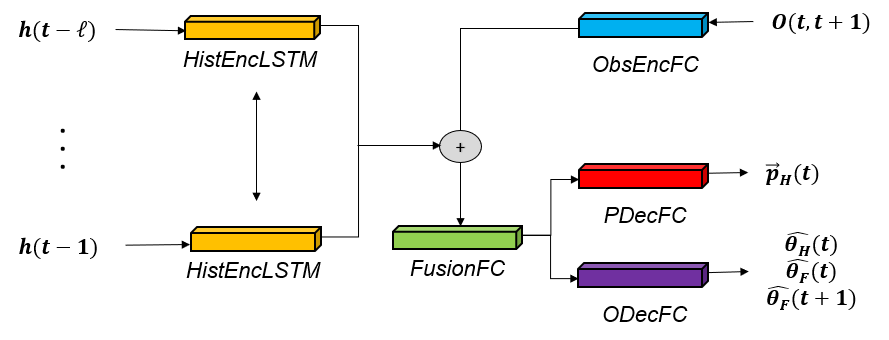
\includegraphics[width=1.\columnwidth]{fig_DL_Pipeline}
		\caption{Structure of our proposed deep neural network.
			This is an snapshot example when applied to a focused module of
			$3$~robots, called \emph{Tail, Follower, Head} within it, at time $t+1$.
            The Encoder--Decoder structure encodes: 1) historical
            positions and orientations of \emph{Follower} and \emph{Head}
            until $t-1$, and 2) the observed positions of the \emph{Follower} at
            $t$ and $t+1$. The decoder part learns to estimate: 1) the
            position of \emph{Head} at $t$, and 2) orientations of
            \emph{Follower} at $t$ and $t+1$ and \emph{Head} at $t$.
		}
		\label{fig:DL_Pipeline}
	\end{figure}
	%
    In addition to the more powerful deep-learning pipeline, we also
    make use of a more realistic robotic platform than in our previous
    work. Previously, we conducted all demonstrations on computer
    simulations, but in this work, we implement our approach in a
    realistic and reproducible physical environment realized by a widely
    available two-wheeled robotic platform, \emph{Thymio}~\cite{Shin14}.

%	All codes are available online\footnote{http://www.github.com/ctyeong}, and supplementary videos
%	are submitted as well.

    This paper is organized as follows. In
    Section~\ref{sec:related_work}, we explore related literature and
    the distinction of our work. Section~\ref{sec:retlo_problem} explains
    more details about our setting of ReTLo problem. Then, we introduce
    our proposed deep-learning solution method in
    Section~\ref{sec:method}. In Section~\ref{sec:experiments}, we
    provide details about experiments performed on real robots,
    including data collection and hyperparameters used for learning. We
    then summarize experimental results in Section~\ref{sec:results}.
    Lastly, we summarize our research and discuss future directions in
    Section~\ref{sec:discussion_and_future_work}.

	\section{Related work}
	\label{sec:related_work}

    In this section, we discuss results from the multi-robot
    systems literature similar to ours and elaborate on the distinct
    contribution of our work. We conclude this section with an
    elaboration of the differences between our results here and our
    previously presented work.

    \subsection{Cooperative localization and tracking}

    Although the ReTLo problem is superficially similar to other known
    cooperative localization and tracking problems~\cite{GKD04, LSRB16,
    FSDO10, CX14, DMG15}, such as cooperative SLAM, it is a distinct
    from general robotic localization. In ReTLo, the robot does not
    execute predictions on its own location but on its teammates using
    accessible information. Moreover, in contrast with cooperative
    localization approaches, robots in ReTLo are assumed to be
    communication free and thus not allowed to communicate with other
    members during the prediction of positions. Hence, in lieu of direct
    signalling, an underlying assumption of the ReTLo problem is that the
    robot behaviors are correlated with the state of the environment
    around them and thus contain cues about the state of their
    neighbors. In this sense, state observers in a networked robotic
    system are more similar to ReTLo than robotic
    localization~\cite{XNX10, GACM12}, but ReTLo does not depend upon
    knowledge of the structure of the underlying robotic controllers and
    does not require that robots move according to simplistic,
    analytically tractable dynamical models. Furthermore, we emphasize
    ReTLo solutions focused on scaling from training with small teams to
    implementation in potentially much larger and possibly variably
    sized teams.

	\subsection{Group state recognition}
	\label{sec:group_state_recognition}

    The ReTLo problem aims to infer the positional state of an entire
    multi-robot team using only locally obtainable information in the
    aspect of a robot member. This is because the knowledge about global
    configuration could help make a better decision for the sake of
    whole team. In this spirit, Brown and Goodrich~\cite{BG14} as well
    as Berger et al.~\cite{BSB16} show that local interactions of robots
    within a swarm can be used to classify swarm-level macroscopic
    structures, such as particular swarm-level shapes like \emph{flock}
    and \emph{torus}. In contrast, our work is to estimate the pose of
    robots themselves, which are the microscopic elements of the
    multi-robot team. Consequently, we make inferences on a space with
    far more degrees of freedom and require a more powerful regression
    model.

	\subsection{Behavioral cue interpretation}
	\label{sec:behavioral_cue_interpretation}

    In the ReTLo problem, the pose of remote robots is to be inferred from
    the motions of nearby robots performing otherwise nominal behaviors.
    This approach allows information to flow around a multi-robot team
    without traditional communication modalities for explicit
    signalling, such as radio communication. Motivated by similar
    constraints on reducing the use of these modalities, Novitzky at
    el.~\cite{NPCBW12} and Das et al.~\cite{DCV16} showed how robots
    performing a special behavior, similar to a ``waggle dance'' of
    honeybees~\cite{VonFrisch67}, could convey information visually or
    mechanically to remotely observing robots. Their approaches are
    different from ours in that we do not require robots to deviate from
    their normal behaviors for the purposes of explicit communication;
    we infer positions only from the latent information in nominal robot
    behavior and interactions.

	\subsection{Robot dynamics learning}
	\label{sec:robot_dynamics_learning}

    Byranvan and Fox~\cite{BF17} proposed a deep learning approach to
    predict the next visual frame given both a current visual frame as
    well as knowledge of a force acting on an object within the frame.
    One of the motivations for this work was to understand the dynamics
    of robotic arms and the relationship with control commands possibly
    executed. In the ReTLo problem described in Section~\ref{sec:intro},
    the \emph{Tail} robot may have accumulated a global shape of robot
    team over time, and it has to be able to predict the future
    formation as a new observation on its neighbor is provided, which
    could be viewed as gaining knowledge of an applied force on the
    team. Such a similarity inspired the architecture of our neural
    network model, but Byranvan and Fox focused on learning motions of
    rigid objects, while a chain of robots in our work can present much
    flexibility in team shape. In addition, the positional information
    about the nearest neighbor is only loosely analogous to the perfect
    knowledge of force used in the frame-prediction example.
    Consequently, our approach is a significant deviation from the one
    proposed by Byranvan and Fox~\cite{BF17}.

	\subsection{Contribution beyond past work}
	\label{sec:scalable_teammate_localization}

    We first presented the ReTLo problem in our previous
    work~\cite{CPR17}. To solve the problem with little robot-to-robot
    communication, the \emph{Tail} robot is designed to use a repetitive
    strategy of inference with which the predictions on a closer robot
    are used as input to prediction for more distant team members. Such
    an approach enables scaling the estimation capability from training
    on small teams to implementation in larger teams without further
    training. We use the same repetitive prediction scheme here;
    however, our focus is now on improving the regression engine to
    broaden its applicability from simulation to physically implemented
    robotic teams using commercially available, off-the-shelf robotic
    platforms.

	\section{ReTLo Problem \& System Design}
	\label{sec:retlo_problem}

    Here, we build on the problem and approach we introduced in our previous
    work~\cite{CPR17}. In particular, we consider a team of $n \in
    \{3,4,\dots\}$ robots designed to move in a line formation.
    Each robot maintains a programmed
    proximity with both the robot ahead of it and behind it, except for
    the \emph{Head} robot that leads the convoy and the \emph{Tail}
    that only follows its single neighbor ahead of it. Each robot in
    between \emph{Head} and \emph{Tail} are referred to as
    \emph{Follower}~$i$, where $i \in \{1, 2, \dots, n-2\}$ represents
    the position relative to the \emph{Tail} (i.e., \emph{Follower}~1 is
    closest to the \emph{Tail}).
%	For better readability, we
%	interchangeably denote the robots as \emph{H, T} and $F_{i}$.

    Every robot has the same sensory and motion capabilities and
    constraints, although they may take different actions according to
    motion rules depending on their roles. This leads to the
    \emph{Follower} and \emph{Tail} robots to behave differently based
    on the current positions of their close neighbors. For simplicity,
    we assume that every robot has an ability to accelerate fast enough
    to always keep the neighbors within their sensory range.

    The ReTLo is to localize all teammates from the view of \emph{Tail}
    only using locally observable information of the position
    of \emph{Follower}~$1$ at every time step. Here, we introduce a 
    more generalized version of ReTLo than in \cite{CPR17} by assuming 
    that until a specific time instant $\tau$, all the information about
    positions and orientations of all robots have been shared reliably 
    with the \emph{Tail} robot, possibly via global communication, albeit
    continued information sharing is unavailable after time $\tau$ thus
    requiring \emph{Tail} to use this localization technique to extrapolate
    from the previously known reliable positions. One can treat our previous
    scenario in \cite{CPR17} as a special case in which  after $\tau$, 
    the \emph{Tail} does not utilize historical information of 
    its teammates and only relies on transient observations of 
    \emph{Follower}~1.

    Formally, at the time instant $\tau$, the following set of poses of
    all teammates is available:
    %
	\begin{equation}
		\{\vec{p}_{r@t},\theta_{r@t}\} \\
	    \label{eq:pose_set}
	\end{equation}
    %
    where $\vec{p}_{r@t} \triangleq (x_{r@t}, y_{r@t})$ is the position
    of robot~$r$ at time~$t$ and $\theta_{r@t}$ is the orientation of
    robot~$r$ at time $t$, with $r \in \{T, F_{1}, F_{2}, ..., F_{n-2},
    H\}$ and $t \leq \tau$. The ReTLo problem is thus, at each time $t >
    \tau$, to observe the position of $F_1$, $\vec{p}_{F_{1@t}}$, and
    use all available information to predict the pose set in
    Eq.~\eqref{eq:pose_set} for time $t'$ where $ \tau < t' \leq t$.

%	This may simulate some realistic scenarios where
%	an unexpected technical issue occurs at a time point disabling any robot-to-robot
%	data transfer, or the robot team intentionally stops the information
%	sharing when entering some specific regions either for security or for saving on the
%	communication cost.

	\section{Proposed Model}
	\label{sec:method}

    Here, we first briefly review our scalable 3-to-many prediction
    approach for training with a small team and implementation on a
    larger team without additional training~\cite{CPR17}. Then in
    Section~\ref{sec:regression_model}, we present our improved
    regression approach that uses not only current nearest-neighbor
    observations but also sequences of past team formations.

    \subsection{Scalable, modular prediction approach}
	\label{sec:scalable_prediction}

    The scalable ReTLo implementation we previously
    introduced~\cite{CPR17} iteratively applies predictions of farther
    and farther robots within focal 3-robot teams, starting with the
    nearest \emph{Follower} robots and eventually leading to prediction
    of the \emph{Head}. In particular, \emph{Tail} initially uses all
    available information about \emph{Follower}~1 at time $t > \tau$ and
    $t+1$ to predict $\vec{p}_{F_2@t}$ of \emph{Follower}~2. Then,
    at $t+2$, \emph{Tail} may repeat this approach centered on
    \emph{Follower}~2 to predict $\vec{p}_{F_3@t}$ of
    \emph{Follower~3}. Thus, after $n-1$ iterations of this approach,
    the \emph{Tail} will eventually have an estimate of the position
    $\vec{p}_{H@t}$ of \emph{Head} at time $t$.

    Because each inference is only applied in 3-robot teams (i.e.,
    the \emph{Tail}, a focal \emph{Follower}, and the robot
    immediately ahead of that \emph{Follower}), the predictor can be
    trained simply with a $3$-robot team and used for a larger size time
    without additional training for the larger-team case.
    However, this iterative modular-prediction approach brings about a
    time delay in making a prediction for a far robot. Furthermore, any
    estimation errors tend to accumulate, making the use of this
    approach limited either to short chains of robots or short
    estimation time periods. Thus, in the next section, we describe a
    regressor significantly improved over our previous
    version~\cite{CPR17} that increases the feasibility of using this
    approach in realistic multi-robot teaming scenarios.

	\subsection{Improved regression model}
	\label{sec:regression_model}

    Because the learned regressor is designed to work in a modular team
    of $3$ robots, notations for robot~$r \in \{H, F, T\}$ only indicate
    the identities of \emph{Head}, \emph{Follower}, and \emph{Tail} and
    not any additional intermediate \emph{Follower} robots. In addition,
    all positions noted here are assumed to be expressed in the
    reference frame of the \emph{Tail} robot because, in practice, the
    \emph{Tail} has to understand positions of others by projection onto
    the local coordinate system centered at itself. Though a similar
    conversion may be considered for orientation, we use absolute
    direction in this work (i.e., assume that all robots agree on
    compass directions) for simplicity.

    In this work, we use a significantly different deep neural network
    architecture than our previous ReTLo work~\cite{CPR17}. As shown in
    Fig.~\ref{fig:DL_Pipeline}, our proposed model uses not only the
    current observation of the follower as an input but also a
    historical sequence of poses. We deconstruct the architecture here.
    %
    \begin{itemize}
        \item We use a fully~connected(FC) layer $f_{obs}$ of size~$k
            \in \mathbb{N}$ to encode
            observations into a feature vector $o \in \mathbb{R}^k$.
            That is,
            %
            \begin{equation}
                o = f_{obs}(X_{obs})
            \end{equation}
            %
            where $X_{obs} = (\vec{p}_{F@t},\vec{p}_{F@t+1})$ is the
            observed positions of \emph{Follower} at times $t$ and $t+1$.

        \item A historical sequence of poses is encoded by a
            bi-directional LSTM layer~\cite{Wu16},
            %
            \begin{equation}
                h = f_{hist}(X_{hist})
            \end{equation}
            %
            where $f_{hist}$ is a LSTM layer, $X_{hist} =
            (\vec{p}_{H@t-\ell:t-1}, \theta_{H@t-\ell:t-1},
            \vec{p}_{F@t-\ell:t-1}, \theta_{F@t-\ell:t-1})$, and $h \in
            \mathbb{R}^{2 \times m}$ is the encoded history feature
            where $\ell$ is the length of historical sequence, and $m$ is
            the size of LSTM layer.

        \item The $o$ and $h$ feature vectors are synthesized by a layer
           $\phi$, which is passed as input to two separate final
           regressors, $g_{p}$ and $g_\theta$, such that
            %
            \begin{equation}
                \begin{split}
                Y_{p} = g_{p}(\phi(o, h)),\\
                Y_{\theta}= g_{\theta}(\phi(o, h))
                \end{split}
                \label{eq:regression_output}
            \end{equation}
            %
            where $Y_{p} = \hat{\vec{p}}_{H@t}$ and $Y_{\theta} =
            (\hat{\theta}_{F@t}, \hat{\theta}_{H@t},
            \hat{\theta}_{F@t+1})$.

            For fusion of $o$ and $h$ features, layer $\phi$ in
            Eq.~\eqref{eq:regression_output} could be implemented by any
            type of layer. During our experiments, we built a FC layer
            of size $d \in \mathbb{N}$ to find a nonlinear relationship
            between the input features and achieved a satisfactory
            performance.

            Furthermore, orientation estimate $\hat{\theta}_{F@t+1}$
            gained with $\hat{\theta}_{F@t}$ is estimated again when
            $\hat{\theta}_{F@t+2}$ is estimated at the next prediction
            step. Although our model keeps the later estimate only, we
            discovered that involving it in both steps can regulate the
            regressor during learning to produce a model that achieves a
            better score in validation.

    \end{itemize}
    %
    To find a best combination of model parameters mentioned above, we
    performed an extensive random search with choices of other learning
    parameters and finally set $k=80, m=160$, and $d=160$.

	\section{Experimental Methodology}
	\label{sec:experiments}

    \subsection{Robotic platform}

    To demonstrate the effectiveness of our method, we employ a
    commercially available, two-wheeled physical robotics platform,
    \emph{Thymio}~\cite{Shin14}, which allows to execute a team of small
    two-wheeled mobile robots. Although each \emph{Thymio} robot has
    sensing and computation capabilities, we used a central computer
    connected with a overhead camera to simulate better proximity
    sensors, more powerful computing power, and a GPS system that would
    be generalizable to other robotic platforms run in a similar
    physical scenario. Specifically, the central system is configured to
    detect the locations of robots in real time using off-the-shelf
    computer vision packages and communicate with a \emph{Raspberry Pi}
    board~\cite{Upton14} mounted on each robot, which implements control
    laws based on the received positional information about neighboring
    robots. The \emph{Tail} and each \emph{Follower} robots were
    configured, as in our previous simulation work~\cite{CPR17}, to
    regulate distance with the robot ahead of it. Regulation of the
    distance behind each \emph{Follower} robot was achieved through
    stopping (as opposed to backward motion), which reduced higher
    frequency oscillations in individual robot motion. Additional
    details about the physical constraints of the laboratory testbed are
    provided in a supplementary video.

    \subsection{Data collection}

    We collected the pose data from two robot teams, one of
    $3$~robots and one of $5$~robots, that ran separately in an arena of
    $2.5 m \times 1.9 m$. The location detection was performed at
    $4$~frames per second at each of which a new command was received by
    each robot. Also, all pose data was collected at the rate of
    $2$~frames per second, which was not necessarily synchronized with
    the command timing. We set the length of history to
    $5$~seconds~($10$~time steps in data recording) and the time window
    for prediction to the next $8$~seconds~($16$~time steps).
       
%    First, the Head robot is initiailized to a random location followed by N-1 robots with roughly a distance of OO cm between neighbors and their random orientations.
    
    We designed a central trajectory planner $\Psi$, which draws random 
    waypoints for \emph{Head} to generate highly arbitrary poses
    of the robot team without frequent human intervention.         
%    which draws a random
%    destination for Head when the robot has reached the previous
%    destination so that the team of robots can provide 
    $\Psi$ is essentially set to simulate a virtual rectangular grid $G$ 
    of "$36 \times 36$" cells, denoted as $c_1, c_2, ..., c_{36}$, 
    overlaid on the physical arena and also operate an array of 
    memory $M$ maintaining indices of the "two" cells most recently 
    visited by the \emph{Head}, with the latest at $M[0]$ and the earlier 
    at $M[1]$. Immediately after the \emph{Head} has reached its destination, 
    for calculating the next waypoint, $\Psi$ first determines candidate
    cells $c_i$ such that $i~\notin~M$ and $A(M[0],i)=1$ where $A(j,k)$ is
    the adjacent matrix of $G$ returning either $1$ if $c_j$ and $c_k$ are
    adjacent geographically or $0$ otherwise. 
    Then, a random coordinate is drawn as the next destination by uniform
    distribution across all the regions of the candidate cells, 
    as shown as red points ahead of the moving team in Fig.~\ref{fig:preds}. 
    As a result, with the wheel speeds in our implementation, 
    the \emph{Head} robot appeared to trigger $3$~times of destination 
    change roughly during the inference time period of $8$~seconds.
    
    Table~\ref{table:data_description} provides details about the
    collected data, where a \emph{Sample} refers to a set of coordinates and
    orientations in a 3-robot group with which a prediction can be
    performed, and an \emph{Instance} is set of all available samples
    for $13$~seconds from the entire team. To reduce temporal
    autocorrelation to help ensure independence of instances, we
    clustered recordings so that instances are separated by at least
    $7$~seconds. All the collected data is open to the 
    public\footnote{https://github.com/ctyeong/ReTLo}
    to encourage more future works on ReTLo.
    %
	\setlength{\tabcolsep}{0.5em} % for the horizontal padding
	{\renewcommand{\arraystretch}{1.2}% for the vertical padding
		\begin{table}[t]
			\centering
			\begin{tabular}{|c|c|c|c|c|}
				\hline
							&  Duration & Num. of Samples & Num. of Instances  \\ \hline
				$3$ robots & $100.6$ minutes & $6,975$ & $465$  \\ \hline
				$5$ robots & $45.0$ minutes  & $8,736$ & $208$  \\ \hline
			\end{tabular}
			\caption{Description of data collected from executions of $3$-robot and $5$-robot teams.}
			\label{table:data_description}
		\end{table}
	}

    \subsection{Model training and performance evaluation}

    Our model is implemented in the \emph{Tensorflow} \emph{Python}
    library\footnote{https://www.tensorflow.org/} to realize the entire
    pipeline, and it was trained to minimize loss functions such as
    Euclidean distance and mean absolute errors for position and
    orientation estimation, respectively. $60$\% data from the $3$-robot
    team is used to train our model, and another $10\%$ was set aside
    for validation. At each epoch of training, a validation followed so
    that the learned weights that achieved the best validation
    performance were saved. The rest of $20\%$ data and all the data
    from $5$-robot were used to test the model. We compare our proposed
    model to two different alternative approaches:
    %
	\begin{itemize}
		\item \emph{$2$X Heuristic}:
            The prediction on \emph{Head} within a modular subteam is
            performed by doubling the vector $\vec{p}_{F} -
            \vec{p}_{T}$.

		\item \emph{FC}:
            Two fully connected layers run in the predictor without
            historical information, which is based on our previous
            proof-of-concept work~\cite{CPR17}.

	\end{itemize}

    \section{Results}
    \label{sec:results}

	\subsection{Overall performance}
	\label{sec:overall_performance}

    In Fig.~\ref{fig:macro_eval}, we compare the averaged error for
    position predictions of the three models in both the $3$-robot and
    $5$-robot team cases. In the case of $3$~robots, the average error
    is calculated only on the prediction for the \emph{Head} robot,
    while in the $5$-robot case, it involves all predictions for
    \emph{Follower 2}, \emph{Follower 3}, and \emph{Head}. Moreover, for
    every model except the \emph{2X Heuristic}, the mean performance of
    $5$~separate learning sessions is reported with the standard
    deviation.
    %
	\begin{figure}[t]
        \centering
        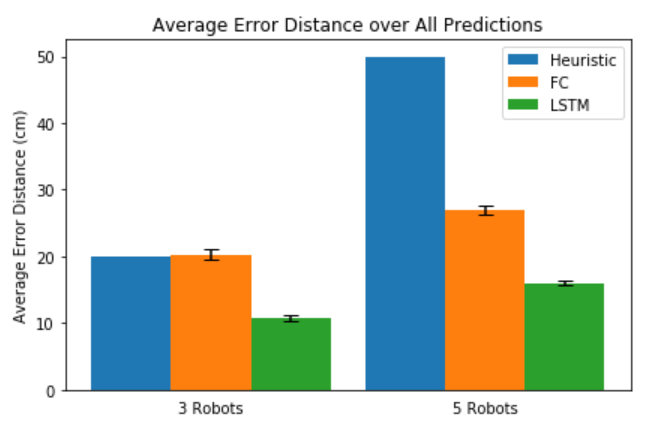
\includegraphics[width=1.\columnwidth]{fig_macro_eval}
        \caption{Average accumulated error of each model in two different sizes of robot team.
            For each of machine learning methods, the mean performance of $5$~separate training
            sessions is reported with a error bar to visualize the performance variation.
        }
        \label{fig:macro_eval}
	\end{figure}

    Figure~\ref{fig:macro_eval} shows that the machine learning methods
    outperform the \emph{2X Heuristic} in any case. In particular, the
    performance gap between \emph{2X Heuristic} and \emph{FC} becomes
    much larger in $5$-robot case suggesting that realistic
    stochasticity presents a significant challenge to the
    straightforward \emph{2X Heuristic} case. Furthermore, our model
    clearly shows the performance improvement over the \emph{FC} model,
    since the average error was reduced by $47\%$ and $40\%$ in the
    $3$-robot and $5$-robot case, respectively. In addition, considering
    the diameter of a \emph{Thymio} robot is $12$~cm, as only three
    robots are deployed, the average distance between the prediction and
    the true position is shorter than the length of the robot body. This
    overall result proves the effectiveness of encoding a sequence of
    historical behaviors as a feature input over the model fed only with
    very recent observation.

	\subsection{Microscopic analysis}
	\label{sec:microscopic_analysis}

    In this section, we analyze the performance of the machine-learning
    based models from a more fine-grained perspective. For each model,
    Fig.~\ref{fig:micro_eval} visualizes the step-wise error for
    different target robots~(i.e., \emph{Follower 2} and \emph{Head}) in
    $5$-robot case, which is calculated by averaging the errors of each
    step across instances. By doing so, we can better understand the
    approximate time frame within which estimation error stays below an
    acceptable error level. During this evaluation, we also had
    $5$~separate training sessions to gain the mean and the variability
    of the performance.
    %
	\begin{figure}[t]
		\centering
		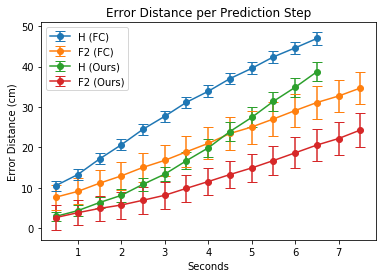
\includegraphics[width=1.\columnwidth]{fig_micro_eval}
		\caption{Average step-wise error for different target robots in $5$-robot team.
			For each model, all the prediction errors at different time steps are averaged
			for a specific robot. The error bars represent the standard deviation of
			$5$~separate models in terms of the performance metric. For the sake of
			visualization, the error for \emph{Follower~3} is omitted, but note that
			in any model, the error ranges between the two visualized errors at every step.
		}
		\label{fig:micro_eval}
	\end{figure}

    Figure~\ref{fig:micro_eval} shows that for any target robot, the
    error increases over time due to the design of the repetitive
    prediction method where previous errors would negatively impact the
    prediction power for the following steps. In a similar sense, each
    model brings about larger error on the \emph{Head} prediction than
    on the \emph{Follower 2}. However, at every time step, our approach
    causes less error than the \emph{FC} model for any robot, and the
    visualized error bars confirm that the performance improvement of
    our approach is significant in every case. Especially for first $4$
    seconds, the prediction on \emph{Head} from our model appears more
    accurate than the prediction on \emph{Follower~2} from the \emph{FC}
    implying that until then, our method also has less error for the
    estimate of \emph{Follower~3} as well. Having said that, the more
    rapid increase in error of our method for the position of
    \emph{Head} may highlight the liability of relying more on prior
    information for future predictions. Nevertheless, these results
    demonstrate the potential of our approach to reduce the
    communication bandwidth necessary for a multi-robot team to perform
    localization.

	\subsection{Qualitative results}
	\label{sec:qualitative_results}

    Figure~\ref{fig:preds} shows images of three different instances of
    $5$-robot team in which both the true positions of all robots and
    the predictions on them are represented. The triangles indicate the
    true positions and orientations, where the yellow triangle is the
    \emph{Tail} and the red triangle is the \emph{Head}. The circles
    indicate the estimated positions of the two farthest \emph{Follower}
    robots as well as the \emph{Head}.
    %
	\begin{figure*}[t]
		\centering
		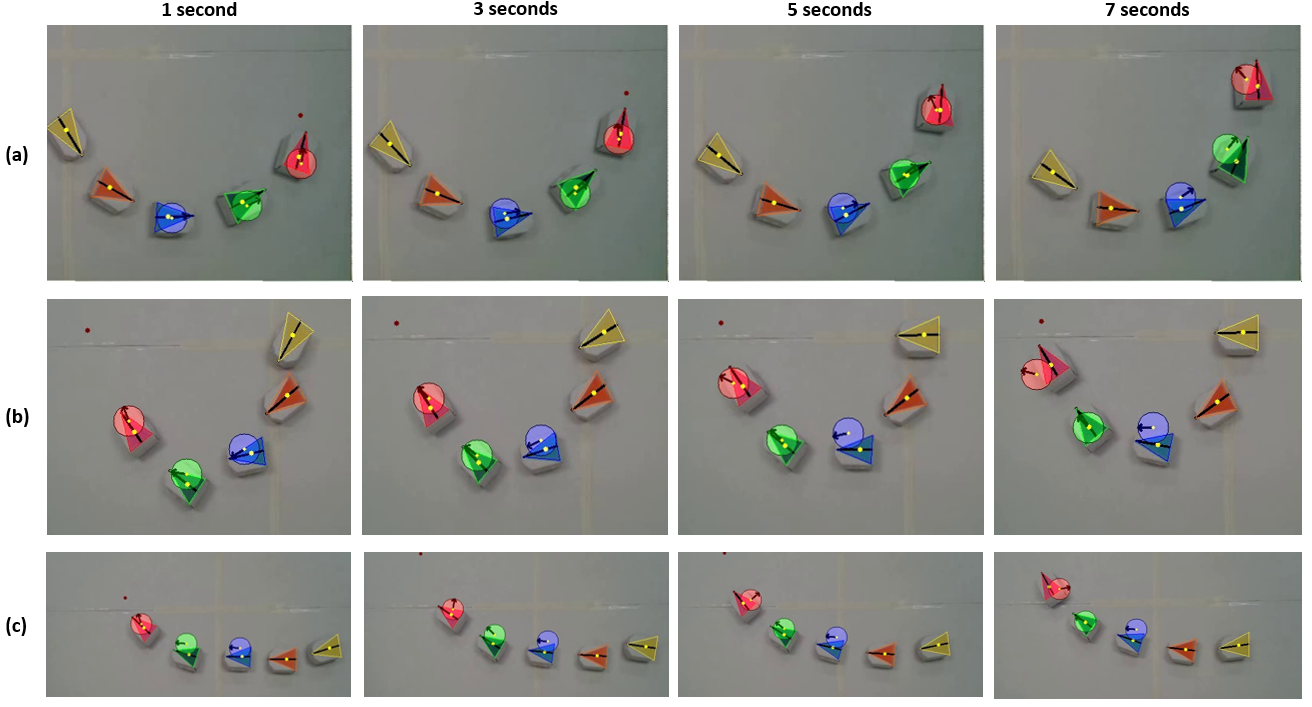
\includegraphics[width=2.\columnwidth]{fig_preds}
		\caption{Sample video frames with prediction results of our proposed model
			for three different instances of $5$~robot team.
			Each row presents four frames of an instance for first $4$~seconds.
			The yellow robot is \emph{Tail}, the pink is \emph{Head}, and
			in-between are \emph{Follower} robots.
			The colored circles are predicted position outputs, in each
			of which a black arrow is drawn to indicate the predicted orientation as well.
			The colored triangles with a black line through the center are the
			results of localization detection used in data collection stage.
			A small red dot on the arena in each frame is the random destination the
			\emph{Head} is moving toward, which is re-sampled at intervals.
		}
		\label{fig:preds}
	\end{figure*}
    %
    Predictions until $4$~seconds are shown to be
    reliable, although there are some errors while the group of robots
    is turning with a high angle and when the \emph{Head} changes its
    destination. Predictions tend to be biased more toward the inside of
    the curve the team is moving on. Unexpectedly, at any instant of
    time, the maximum position error is often at intermediate
    \emph{Follower} robots and not at the most distant \emph{Head}
    robot. Such corrections may be the result of using historical
    information to constrain the possible locations of farther robots,
    as in data fusion techniques that use formal dynamical models to
    physically constrain estimator variance. However, our approach does
    not make use of explicit formal dynamical models.

	\section{Summary \& Future work}
	\label{sec:discussion_and_future_work}

    By formally incorporating historical data into the design of a
    scalable, localization regression module, we have improved upon our
    previous work~\cite{CPR17} in estimating the positions of robots in
    a multi-robot team using only observations of a single, nearest
    neighbor robot. As in our previous model, the regression module we
    design can be trained on small teams of 3 robots and generalize to
    larger teams with no additional training. However, our new approach
    greatly reduces estimator error, giving it the potential to greatly
    reduce communication bandwidth in other localization schemes that
    otherwise require continuous communication among robots.

    To test our approach, we utilized a commercially available robotic
    platform, \emph{Thymio}, to collect datasets from $3$-robot and
    $5$-robot teams. Through empirical experiments, we showed that the
    proposed machine learning model offers more accurate estimation than
    other approaches. We analyzed our estimator performance over time
    and demonstrated its improved performance for short horizons but
    potential added liabilities for longer time horizons. Lastly, we
    overlayed visualizations of the prediction outcomes on images of the
    actual robotic system to illustrate specific cases where low
    estimation error was provided for far-away robots despite high error
    on more nearby robots.

    In the future work, we could more deeply investigate the factors in
    model accuracy such as the length of history or types of team
    behavior that might favor the prediction scheme. Also, because the
    LSTM layer is exposed to various evolutions of team shape during
    training, the vector representation of it may be examined to
    characterize team states and ultimately detect large-scale
    group-shape abnormalities that may be important to detect for
    situational awareness. Beyond these approaches, we are currently
    working toward Bayesian implementations that make better use of
    uncertainty information from sensors and provide confidence
    estimates for the position of each robot in the team. Such
    approaches, when incorporated into a framework such as partially
    observable Markov decision processes, could lead to approaches for
    using actuation (as opposed to communication) to reduce estimator
    error.

{\small
	\bibliographystyle{IEEEtran}
	%\bibliography{IEEEabrv, IEEEexample}
	\bibliography{IEEEexample}
}

\end{document}
